\documentclass[tikz,border=2mm]{standalone}
\usepackage{amsmath}

\begin{document}
    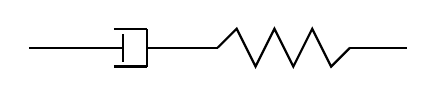
\begin{tikzpicture}[line width=1pt,scale=1.2]

        % Draw the input line
        \draw[thick] (-2,0) -- (-1,0);

        % Degenerated damper (one side inside)
        \draw[thick] (-1,-0.15) -- (-1,0.15); % Vertical line
        \draw[thick] (-1.1,-0.2) -- (-0.75,-0.2); % Bottom horizontal line
        \draw[thick] (-1.1, 0.2) -- (-0.75, 0.2); % Upper horizontal line
        \draw[thick] (-0.75, -0.2) -- (-0.75, 0.2); % Middle vertical line
        \draw[thick] (-0.75, 0.) -- (0, 0.); % Middle horizontal line
        %\draw[thick] (-1,0.3) -- (0,0);     % Diagonal line connecting top to middle

% Spring with three zigzags
        \draw[thick] (0,0) -- (0.2,0.2) -- (0.4,-0.2) -- (0.6,0.2) -- (0.8,-0.2) -- (1,0.2) -- (1.2,-0.2) -- (1.4,0);

        % Output line
        \draw[thick] (1.4,0) -- (2,0);

    \end{tikzpicture}
\end{document}
